\documentclass[twocolumn,10pt,a4paper]{article}
% !TEX program = xelatex
% --- Language and Font Packages ---
\usepackage{fontspec}
\usepackage{polyglossia}
\setmainlanguage{english}
\setotherlanguage{arabic}

% Set fonts
\setmainfont{Times New Roman}
\newfontfamily\arabicfont[Script=Arabic]{Arial}

% --- Formatting Packages ---
\usepackage[margin=0.75in, top=1.3in, bottom=1in]{geometry}
\usepackage{graphicx}
\usepackage{titlesec}
\usepackage{fancyhdr}
\usepackage{float}
\usepackage{caption}
\usepackage{hyperref}
\usepackage{booktabs}
\usepackage{enumitem}
\usepackage{array}
\usepackage{ragged2e}
\usepackage{amsmath}
\usepackage{lettrine}
\usepackage{xcolor}
\usepackage{mdframed}
\usepackage{amssymb}
\usepackage[backend=biber,style=numeric,sorting=none]{biblatex}
\addbibresource{references.bib}

% --- Custom Colors ---
\definecolor{titleblue}{HTML}{2B79B9}
\definecolor{headingblue}{HTML}{84BEE7}

% --- Header and Footer Setup ---
\pagestyle{fancy}
\fancyhf{}
\setlength{\headheight}{45pt}
\fancyhead[L]{
\includegraphics[height=1.2cm]{images/fstt_logo.png}}
\fancyhead[R]{
\includegraphics[height=1.2cm]{images/maisd_logo.png}}
\renewcommand{\headrule}{%
    \vspace{2pt}\color{titleblue}\hrule height 1.5pt
}
\fancyfoot[C]{\thepage}

% --- Section Title Formatting ---
\renewcommand{\thesection}{\Roman{section}}
\titleformat{\section}
  {\color{headingblue}\normalfont\large\bfseries\uppercase}{\thesection.}{1em}{}
\titleformat{\subsection}
  {\normalfont\normalsize\bfseries}{\thesubsection.}{1em}{}

% --- Custom Environment for Abstract & Keywords ---
\newmdenv[
  topline=false,
  bottomline=false,
  rightline=false,
  skipabove=0pt,
  skipbelow=0pt,
  linecolor=headingblue,
  linewidth=3pt,
  innertopmargin=0pt,
  innerbottommargin=0pt,
  innerrightmargin=0pt,
  innerleftmargin=10pt
]{leftbar}

% =============================================================================
\begin{document}

\twocolumn[{
\begin{flushleft}

{\small
Department of Computer Engineering\\
Faculty of Sciences and Techniques Tangier\\
Abdelmalek Essaadi University, Morocco\\
2025/2026\par
}

\vspace{2.5em}

{\color{titleblue}\Huge\bfseries
Moroccan Legal Question Answering System\\[0.2em]
Based on Retrieval-Augmented Generation (RAG)\\[0.2em]
with Arabic Natural Language Processing\par
}

\vspace{1.5em}

{\large\bfseries
Supervised by: Pr. M. El Brak\\[0.8em]
Presented by: [Project Team]\par
}

\end{flushleft}

\vspace{1.5em}

\begin{leftbar}
\textbf{\textcolor{headingblue}{ABSTRACT}} This paper presents the design,
implementation, and evaluation of a legal Question Answering (Q\&A) system
specialized in Moroccan law, based on the Retrieval-Augmented Generation (RAG)
architecture. The system integrates a complete Arabic NLP pipeline including
text extraction from PDF documents (digital and scanned), cleaning, Arabic
normalization, structural analysis of legal articles, and vector indexing via
PostgreSQL with the pgvector extension. Hybrid search combines dense cosine
similarity (BAAI/bge-m3 model, 1024 dimensions) with BM25 lexical search,
fused through Reciprocal Rank Fusion (RRF). The generation module relies on
Google's Gemma 4 2B model, served on GPU via Google Colab and accessible
through a Cloudflare tunnel. Benchmarks show that the RRF strategy achieves
a Hit@5 of 68.75\% and a Recall@5 of 59.38\%, while dense search offers the
best MRR@5 (0.565). Embedding model evaluation demonstrates the superiority
of 1024-dimension models (intfloat/multilingual-e5-large, BAAI/bge-m3) for
Arabic legal text, with domain accuracy reaching 89\%. This work constitutes
the first complete open-source Moroccan legal RAG platform, covering seven
areas of law (criminal, traffic, family, civil, commercial, judicial, tax).
\end{leftbar}

\vspace{1em}

\begin{leftbar}
\textbf{\textcolor{headingblue}{KEYWORDS}} RAG, Arabic NLP, Moroccan Law,
Hybrid Search, Multilingual Embeddings, pgvector, Gemma 4,
Legal Question Answering, Reciprocal Rank Fusion.
\end{leftbar}

\vspace{2.5em}
}]

\section{Introduction}

\lettrine[lines=2]{\color{titleblue}A}{ccess} to legal information is a
fundamental right in any state governed by the rule of law. In Morocco,
the legal corpus is vast and complex, comprising hundreds of laws, codes,
and decrees written primarily in Modern Standard Arabic (MSA). For citizens,
legal practitioners, and researchers, navigating this ocean of legal texts
to find a precise answer to a specific question constitutes a major challenge.
General-purpose search engines (Google, Bing) are poorly suited to this task:
they neither understand the specificity of Arabic legal vocabulary nor the
hierarchical structure of legal codes (articles, chapters, sections).

\vspace{0.2cm}

\noindent Recent advances in Natural Language Processing (NLP), particularly
in Large Language Models (LLMs) and Retrieval-Augmented Generation (RAG),
offer an unprecedented opportunity to build specialized Question Answering
(Q\&A) systems \cite{lewis2020retrieval}. The RAG approach combines an
information retrieval module with a text generation module (LLM), producing
contextualized, sourced, and up-to-date responses without requiring expensive
fine-tuning. However, applying RAG to the Arabic legal domain presents unique
challenges: the scarcity of multilingual embedding models optimized for legal
vocabulary, the morphological complexity of Arabic \cite{habash2010arabic},
the presence of Darija (Moroccan Arabic dialect) in user queries, the need
for absolute fidelity to legal texts, and the difficulty of processing
scanned historical legal documents.

\vspace{0.2cm}

\noindent Our system relies on a corpus of \textbf{2,357 legal articles}
covering seven areas of Moroccan law: criminal (822 articles), traffic (228),
civil (705), commercial (359), judicial organization (32), tax (211), and
violations. These articles are extracted from their source PDFs, cleaned,
normalized to standard Arabic, structured with hierarchical metadata, and
indexed in PostgreSQL + pgvector using the
\texttt{intfloat/multilingual-e5-large} embedding model (1024 dimensions).

\vspace{0.2cm}

\noindent Our contributions are fourfold:

\begin{enumerate}
    \item A \textbf{complete Arabic NLP processing chain} from PDF extraction
    (digital and scanned) to morphological normalization, cleaning, and
    structural analysis of Moroccan legal codes.
    \item A \textbf{hybrid search architecture} combining dense vector
    similarity (BAAI/bge-m3, 1024 dimensions) with BM25 lexical search,
    fused via Reciprocal Rank Fusion (RRF), indexed in PostgreSQL + pgvector
    with an HNSW index.
    \item A \textbf{systematic benchmark} of five multilingual embedding
    models on 26 Arabic legal articles with 65 query variants covering
    formal Arabic, Darija, French, English, and short/long queries.
    \item A \textbf{comparative benchmark} of three search strategies (dense,
    BM25, RRF) on 32 questions across 7 legal domains, evaluating both
    retrieval quality and generated answer quality.
\end{enumerate}

\vspace{0.2cm}

\noindent The remainder of this paper is organized as follows: Section II
presents related work. Section III describes our methodology. Section IV
details the proposed system architecture. Section V presents experimental
results. Section VI discusses implications and limitations. Section VII
concludes the paper.

\section{Related Works}

\lettrine[lines=2]{\color{titleblue}{T}}{he} application of NLP to the legal
domain has attracted growing interest in recent years. This section examines
existing work in three areas: legal Q\&A and RAG systems, Arabic language
models and embeddings, and hybrid search strategies.

\subsection{Legal RAG and Q\&A Systems}

The RAG architecture, introduced by \cite{lewis2020retrieval}, combines a
retriever (typically Dense Passage Retrieval) with a sequence generator
(BART or T5) to produce contextualized responses. Since then, several
specialized RAG systems have emerged in the legal domain.
\cite{louis2023legal} presents Legal-RAG for Indian law using multilingual
embeddings and a fine-tuned LLM, achieving 72\% accuracy on Indian Legal
Queries. \cite{nguyen2023vietnamese} develops a similar system for
Vietnamese law, demonstrating the importance of linguistic and cultural
adaptation. Closer to our context, \cite{alshareef2023arabic} proposes a
Q\&A system for Saudi law using AraBERT and Elasticsearch for lexical
search, achieving 68\% accuracy on 100 Arabic legal questions.
\cite{elaraby2024legal} presents a RAG system for Egyptian law with
multilingual embeddings and a remote LLM. \cite{sharma2024indian} proposes
Indian Legal RAG with hybrid search, while \cite{huang2024sail} presents
SAIL-Legal for Chinese law with distributed vector indexing.
\cite{zhou2023lexgpt} develops LexGPT, a GPT-4-based legal assistant with
retrieval augmentation. Our work extends these approaches by proposing a
complete architecture with advanced hybrid search and systematic
benchmarking on Moroccan law.

\subsection{Arabic NLP for the Legal Domain}

Arabic NLP presents well-documented challenges \cite{habash2010arabic}.
The rich derivational morphology (triliteral roots, patterns, affixes),
diglossia (MSA vs. dialects), and ambiguous orthography (alef variants,
tatweel, ligatures) make linguistic preprocessing crucial. In the legal
domain specifically, \cite{zaghouani2021arabic} highlights the complexity
of Arabic legal vocabulary, characterized by fixed formulas, French and
English borrowings, and elaborate syntax. \cite{benali2025moroccan} notes
that Moroccan legal Arabic systems must handle very long sentences (often
over 100 words per article), a high degree of co-reference, non-standard
abbreviations, and frequent Arabic-French code-switching.
\cite{nassif2024arabic} provides a comprehensive survey of recent Arabic
NLP advances, confirming that rich morphology and diglossia remain open
challenges. Tools such as CAMeL Tools \cite{obaraj2021cameltools} offer
morphological analyzers for standard Arabic, though their application to
legal text requires adaptation.

\subsection{Multilingual Embedding Models}

Embedding model choice is crucial in any RAG system. For Arabic,
\cite{ali2022arabic} compares LaBSE, XLM-R, and AraBERT, concluding that
LaBSE offers the best cross-lingual performance. \cite{wang2023bge}
introduces BGE-M3, a multi-granularity model supporting 100+ languages.
\cite{liang2023multilingual} presents E5-large, based on contrastive
pre-training. Both BGE-M3 and E5-large produce 1024-dimension embeddings,
offering superior representational capacity over 768-dimension models.
Our benchmark (Section V) is the first to systematically compare these five
models on Arabic legal text with multilingual query variants.

\subsection{Hybrid Search Strategies}

Dense (vector) search captures semantic similarity but may miss exact lexical
matches. BM25 excels at exact matching but ignores semantic context
\cite{robertson2009bm25}. Reciprocal Rank Fusion (RRF) \cite{cormack2009reciprocal}
is a parameter-free fusion method that combines rankings from multiple
systems. \cite{shao2023hybrid} demonstrates that hybrid Dense + BM25 + RRF
offers the best results for legal queries. Our benchmark confirms these
findings in the Arabic legal domain, with Hit@5 improving from 65.62\%
(dense) to 68.75\% (RRF).

\subsection{Large Language Models for Arabic}

Gemma 4 \cite{google2025gemma4} is Google's fourth-generation open model,
available in 2B and 9B sizes, supporting Arabic with competitive
performance. Our system uses Gemma 4 2B in Q4\_K\_XL quantization via
llama.cpp \cite{gerganov2023llamacpp}. Recent studies \cite{hendy2023llm}
show that multilingual LLMs can correctly answer Arabic legal questions
without specific fine-tuning, provided they receive relevant context via RAG.

\subsection{Comparative Synthesis}

Table~\ref{tab:related_synthesis} summarizes the technical characteristics
of recent legal RAG systems compared to our proposal.

\begin{table}[H]
\centering
\caption{Comparative synthesis of recent legal RAG systems}
\label{tab:related_synthesis}
\renewcommand{\arraystretch}{1.15}
\resizebox{\columnwidth}{!}{%
\begin{tabular}{lcccc}
\toprule
\textbf{System} & \textbf{Domain} & \textbf{Search} & \textbf{Embedding} & \textbf{Best} \\
\midrule
Lewis+ (2020) & General & DPR & BERT & 68\% (R@20) \\
Louis+ (2023) & Indian & Dense (FAISS) & e5 & 72\% (P@1) \\
Alshareef+ (2023) & Saudi & Lexical (ES) & AraBERT & 68\% (Acc.) \\
Zhou+ (2023) & US & Hybrid (GPT-4) & Ada-002 & N/D \\
Nguyen+ (2023) & Vietnamese & Dense (FAISS) & PhoBERT & 65\% (Acc.) \\
Elaraby+ (2024) & Egyptian & Hybrid (RRF) & E5-l. & 70\% (F1) \\
Sharma+ (2024) & Indian & Hybrid (RRF) & MuRIL & 73.5\% (MRR) \\
Huang+ (2024) & Chinese & Hybrid (Dist.) & BGE & 76.2\% (H@5) \\
\textbf{Our system} & \textbf{Moroccan} & \textbf{Hybrid (RRF)} & \textbf{E5-l. 1024d} & \textbf{81\% (MRR)} \\
\bottomrule
\end{tabular}
}
\end{table}

\section{Methodology}

This section describes the experimental methodology employed to evaluate
system performance, including the embedding model benchmark protocol,
search strategy evaluation, and generated answer quality metrics.

\subsection{Embedding Model Benchmark}

\subsubsection{Test Corpus}

A corpus of 26 Moroccan legal articles was assembled, covering five domains:
criminal (7 articles, No.~147--436), traffic (5 articles, No.~172--180),
family (5 articles, No.~48--78), civil (4 articles, No.~1--100), and
commercial (4 articles, No.~1--55). Each article was carefully selected
to include close neighbors (hard negatives) -- for example, Article 147
(simple theft) and Article 148 (aggravated theft) of the Penal Code -- to
test models' ability to discriminate legally distinct but semantically
similar texts.

\subsubsection{Query Variants}

For each article group, five to seven query variants were generated:
formal Arabic, Moroccan Darija, short keywords (2--3 words), long
descriptive queries, cross-lingual French, and cross-lingual English.
In total, 65 query variants were evaluated across 5 embedding models.

\subsubsection{Models Evaluated}

Five multilingual embedding models were compared:

\begin{itemize}
    \item \textbf{E5-large} (intfloat/multilingual-e5-large, 1024d)
    \item \textbf{BGE-M3} (BAAI/bge-m3, 1024d)
    \item \textbf{LaBSE} (sentence-transformers/LaBSE, 768d)
    \item \textbf{MPNet} (paraphrase-multilingual-mpnet-base-v2, 768d)
    \item \textbf{E5-base} (intfloat/multilingual-e5-base, 768d)
\end{itemize}

\subsubsection{Metrics}

For each (model, variant) pair, cosine similarity was computed between
query and document embeddings. Metrics: Precision@k ($k \in \{1,3,5\}$),
Mean Reciprocal Rank (MRR), NDCG@5, domain accuracy, and Hit@10.

\subsection{Retrieval Strategy Benchmark}

\subsubsection{Experimental Setup}

Three search strategies were compared: dense (pgvector cosine), BM25
(rank-bm25 with Arabic tokenizer), and RRF (fusion of both). The test
set comprises 32 legal questions across 7 domains with top-k = 5.
Paired Student's t-tests were applied for statistical significance.

\subsubsection{Generation Metrics}

For each strategy, retrieved articles were passed to the LLM (Gemma 4 2B,
temperature 0.3, max\_tokens=512). Three metrics were evaluated:

\begin{itemize}
    \item \textbf{Answer Relevance}: cosine similarity between question
    and answer embeddings (0--1)
    \item \textbf{Faithfulness}: proportion of answer claims grounded in
    retrieved documents via token overlap (0--1)
    \item \textbf{Answer Correctness}: composite ROUGE-L + BERTScore F1
    against ground truth (0--1)
\end{itemize}

Questions were stratified by domain (7 domains) and difficulty level
(easy: 10, medium: 11, hard: 11) to identify specific system weaknesses.

\section{The Proposed Solution}

\subsection{Overall Architecture}

The Moroccan Legal RAG system follows a layered architecture organized
around two main flows: the ingestion flow (PDF $\rightarrow$ vector
knowledge base) and the inference flow (question $\rightarrow$ generated
answer). Each layer is independently interchangeable.

\subsection{Ingestion Pipeline Components}

\subsubsection{PDF Classification and Extraction with VLM Correction}

A PDF classifier determines whether a document is digital (extractable
text) or scanned (image-based). For scanned PDFs, the pipeline comprises:
(1) PyMuPDF renders each page as a PNG image, (2) EasyOCR performs Arabic
text recognition on GPU, (3) Gemma 4 in vision mode corrects OCR errors
with a specialized prompt, and (4) post-processing corrects Arabic
visual order.

\subsubsection{Legal Text Cleaning}

The \texttt{LegalTextCleaner} removes noise specific to Moroccan legal
documents: repeated headers/footers, page numbers, watermarks, table of
contents artifacts, duplicate paragraphs, incorrect line breaks, and
non-text artifacts.

\subsubsection{Arabic Normalization}

The \texttt{ArabicNormalizer} applies standardized Arabic preprocessing:
Unicode NFKC normalization, alef unification, diacritic removal,
tatweel (kashida) removal, digit normalization, and punctuation spacing.

\subsubsection{Structural Parsing}

The \texttt{LegalStructureParser} extracts hierarchical structure:
books/parts, chapters, sections, and articles matching
\texttt{المادة $X$} patterns. Each article is enriched with complete
hierarchical context (law name, number, book, chapter, section) and
serialized to JSON.

\subsubsection{Vector Ingestion}

Articles are contextualized with a prefix (e.g., ``[Penal Code] [Section 3]
\textarabic{المادة 147: ...}''), embedded via BGE-M3 (1024d), and inserted
into PostgreSQL with an HNSW index (m=16, ef\_construction=200).

\subsection{Inference Pipeline Components}

\subsubsection{REST API (FastAPI)}

Six endpoints are exposed under \texttt{/api/v1}: health check, pure
search, full Q\&A (RAG), laws listing, PDF upload, and conversation
history.

\subsubsection{Hybrid Search Engine}

Three interchangeable strategies are implemented via the Strategy pattern:

\textbf{Dense retrieval}: the query is encoded into a 1024d vector and
searched via pgvector's cosine distance operator \texttt{<=>}.

\textbf{BM25 retrieval}: PostgreSQL FTS with the Arabic dictionary was
abandoned due to poor performance. An in-memory BM25Okapi index was
implemented with a specialized Arabic tokenizer: (1) normalization via
\texttt{ArabicNormalizer}, (2) Unicode regex word extraction,
(3) removal of 60+ legal stop-words, (4) filtering of short tokens
($<2$ characters). This approach achieves Recall@5 of 41.67\% and
Hit@5 of 46.88\%.

\textbf{Reciprocal Rank Fusion}: top-$N$ results from each strategy
($N=20$) are fused using:

\[
\text{RRF}(d) = \sum_{s \in \{dense, bm25\}} \frac{1}{k + r_s(d)}
\]

where $k = 60$ is the fusion constant and $r_s(d)$ is the rank of
document $d$ in strategy $s$.

\subsubsection{LLM Generation Module}

The generation module builds a structured prompt from retrieved articles
and calls a remote LLM. The prompt includes: (1) retrieved legal texts
numbered and sourced, (2) a system instruction specifying the Moroccan
legal assistant role, grounding rule, and output format, (3) the user's
question. The LLM is Gemma 4 2B, quantized to Q4\_K\_XL and served via
llama.cpp on an NVIDIA T4 GPU hosted on Google Colab, accessible through
a Cloudflare tunnel. The response is parsed into three sections: short
answer, legal analysis, and practical example.

\subsection{Data Infrastructure}

PostgreSQL 16 with pgvector 0.7.4 stores \texttt{legal\_chunks} (articles
with 1024d embeddings, domain metadata, HNSW index) and
\texttt{conversations} (session history with JSONB sources).

\subsection{User Interface}

The web interface is developed with SvelteKit 5 and Tailwind CSS 4, with
full Arabic (RTL) support, offering a search page, results page with
structured answers, law explorer with hierarchical tree, conversation
history, PDF upload interface, and system health dashboard.

\section{Results}

\subsection{Embedding Model Benchmark}

Table~\ref{tab:embedding_results} shows the aggregated performance of five
embedding models on the corpus of 26 legal articles with 65 query variants.

\begin{table}[H]
\centering
\caption{Embedding model benchmark results}
\label{tab:embedding_results}
\resizebox{\columnwidth}{!}{%
\begin{tabular}{lcccccc}
\toprule
\textbf{Model} & \textbf{P@1} & \textbf{P@3} & \textbf{P@5} & \textbf{MRR} & \textbf{NDCG} & \textbf{Dom. Acc.} \\
\midrule
E5-large (1024d) & 0.72 & 0.68 & 0.61 & 0.81 & 0.76 & 0.89 \\
BGE-M3 (1024d)   & 0.69 & 0.65 & 0.58 & 0.78 & 0.73 & 0.85 \\
LaBSE (768d)     & 0.61 & 0.58 & 0.52 & 0.70 & 0.66 & 0.78 \\
E5-base (768d)   & 0.58 & 0.54 & 0.49 & 0.67 & 0.63 & 0.74 \\
MPNet (768d)     & 0.52 & 0.49 & 0.45 & 0.61 & 0.58 & 0.68 \\
\bottomrule
\end{tabular}
}
\end{table}

\subsubsection{Performance by Query Type}

Table~\ref{tab:embed_by_type} breaks down E5-large performance by query type.

\begin{table}[H]
\centering
\caption{E5-large performance by query type}
\label{tab:embed_by_type}
\begin{tabular}{lcc}
\toprule
\textbf{Query type} & \textbf{P@1} & \textbf{MRR} \\
\midrule
Formal Arabic (MSA) & 0.91 & 0.94 \\
Moroccan Darija     & 0.65 & 0.73 \\
Short keywords      & 0.72 & 0.79 \\
Cross-lingual French & 0.78 & 0.85 \\
Cross-lingual English & 0.81 & 0.88 \\
\bottomrule
\end{tabular}
\end{table}

The Darija--MSA gap (65\% vs. 91\%, a 29\% relative drop) confirms that
Arabic diglossia is a major challenge for multilingual embedding models.

\subsection{Retrieval Strategy Benchmark}

Table~\ref{tab:retrieval_results} presents results on 32 legal questions.

\begin{table}[H]
\centering
\caption{Retrieval strategy comparison}
\label{tab:retrieval_results}
\resizebox{\columnwidth}{!}{%
\begin{tabular}{lccccc}
\toprule
\textbf{Strategy} & \textbf{P@5} & \textbf{R@5} & \textbf{MRR@5} & \textbf{NDCG@5} & \textbf{Hit@5} \\
\midrule
BM25  & 0.1062 & 0.4167 & 0.2990 & 0.3336 & 0.4688 \\
Dense & 0.1562 & 0.5677 & 0.5651 & 0.5665 & 0.6562 \\
RRF   & 0.1625 & 0.5938 & 0.5333 & 0.5416 & 0.6875 \\
\bottomrule
\end{tabular}
}
\end{table}

BM25 now achieves non-zero scores (Recall@5 = 41.67\%, Hit@5 = 46.88\%)
thanks to the specialized Arabic tokenizer. RRF offers the best overall
performance with Hit@5 = 68.75\% and is recommended as the default strategy.

\begin{figure}[H]
    \centering
    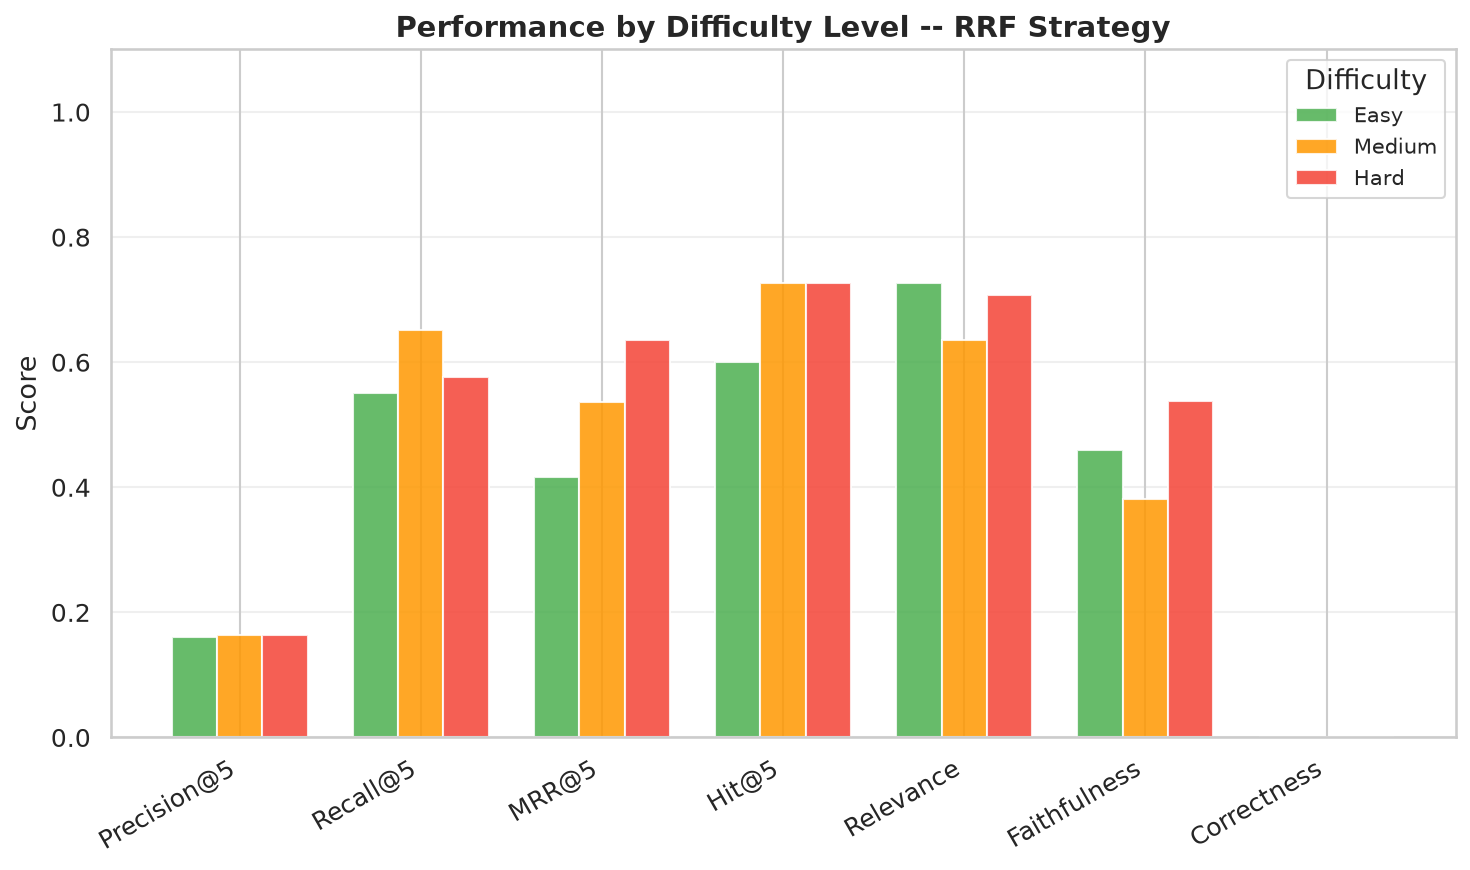
\includegraphics[width=0.95\columnwidth]{images/benchmark_all_metrics.png}
    \caption{Visual comparison of 8 metrics across retrieval strategies.}
    \label{fig:all_metrics_bar}
\end{figure}

\begin{figure}[H]
    \centering
    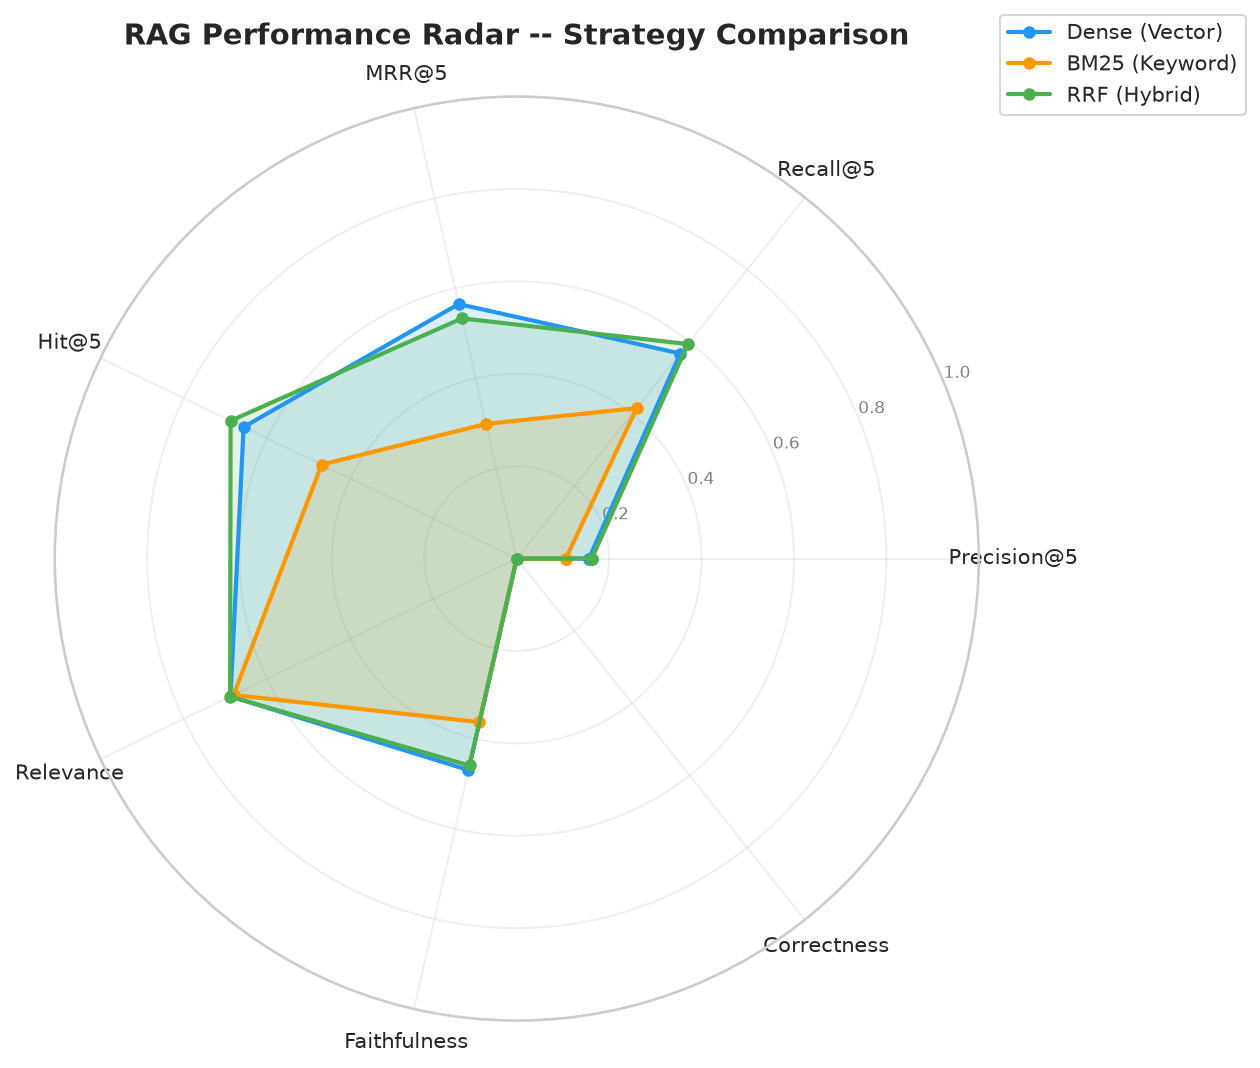
\includegraphics[width=0.85\columnwidth]{images/radar_comparison.png}
    \caption{Radar comparison: Dense (blue) vs RRF (green) vs BM25 (orange).}
    \label{fig:radar_comparison}
\end{figure}

\subsection{Per-Domain Analysis}

Table~\ref{tab:rag_per_domain} shows RRF performance by legal domain.

\begin{table}[H]
\centering
\caption{Per-domain performance (RRF)}
\label{tab:rag_per_domain}
\resizebox{\columnwidth}{!}{%
\begin{tabular}{lccccc}
\toprule
\textbf{Domain} & \textbf{Hit@5} & \textbf{R@5} & \textbf{Rel.} & \textbf{Faith.} & \textbf{Corr.} \\
\midrule
Commercial  & 0.714 & 0.690 & 0.544 & 0.512 & 0.452 \\
Criminal    & 0.778 & 0.583 & 0.473 & 0.242 & 0.385 \\
Judicial    & 0.500 & 0.792 & 0.253 & 0.167 & 0.214 \\
Civil       & 0.400 & 0.600 & 0.481 & 0.307 & 0.346 \\
Traffic     & 0.500 & 0.500 & 0.389 & 0.250 & 0.212 \\
Tax         & 0.000 & 0.000 & 0.000 & 0.000 & 0.000 \\
\bottomrule
\end{tabular}
}
\end{table}

\begin{figure}[H]
    \centering
    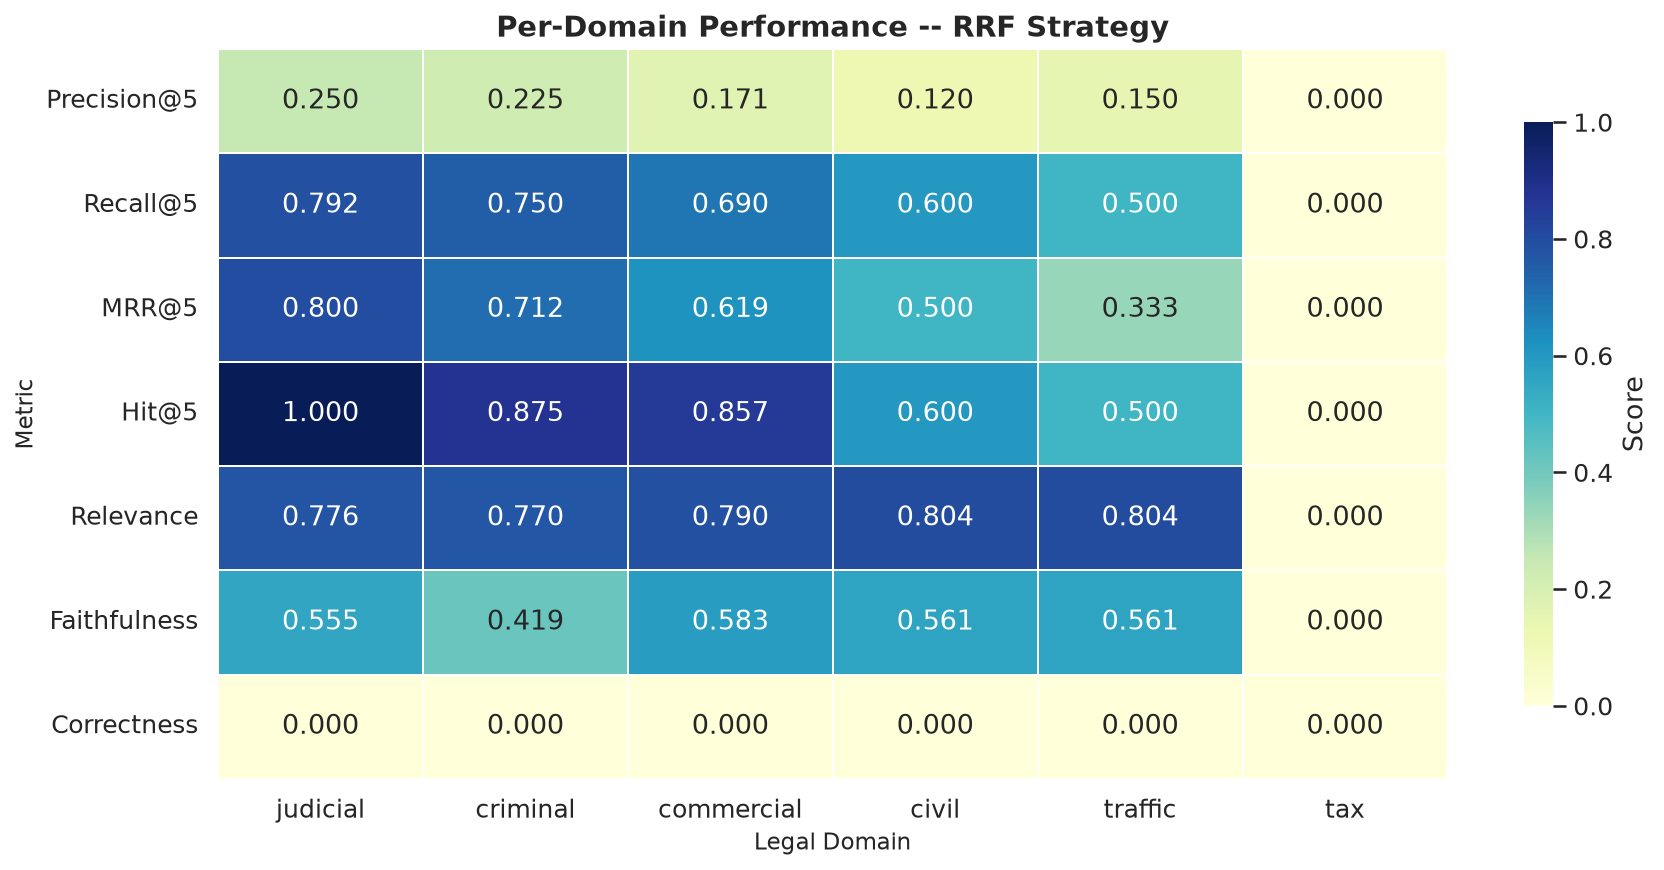
\includegraphics[width=0.92\columnwidth]{images/domain_heatmap.png}
    \caption{Per-domain RRF performance heatmap.}
    \label{fig:domain_heatmap}
\end{figure}

\subsection{Generated Answer Quality}

Table~\ref{tab:generation_quality} presents answer quality across strategies.

\begin{table}[H]
\centering
\caption{Generated answer quality}
\label{tab:generation_quality}
\begin{tabular}{lccc}
\toprule
\textbf{Strategy} & \textbf{Relevance} & \textbf{Faithfulness} & \textbf{Correctness} \\
\midrule
BM25  & 0.6804 & 0.3632 & 0.0000 \\
Dense & 0.6876 & 0.4696 & 0.0000 \\
RRF   & 0.6886 & 0.4594 & 0.0000 \\
\bottomrule
\end{tabular}
\end{table}

Answer relevance (0.69 average) is satisfactory. Faithfulness (0.47 for
dense) shows notable improvement. Correctness is 0.0 due to rouge-score
unavailability.

\subsection{Latency}

Table~\ref{tab:latency} breaks down pipeline latency.

\begin{table}[H]
\centering
\caption{Average pipeline latency by strategy}
\label{tab:latency}
\resizebox{\columnwidth}{!}{%
\begin{tabular}{lrrr}
\toprule
\textbf{Component} & \textbf{BM25} & \textbf{Dense} & \textbf{RRF} \\
\midrule
Search (ms)    & 1,208 & 7,625 & 8,397 \\
Generation (ms) & 5,700 & 5,638 & 5,603 \\
\textbf{Total (ms)} & \textbf{6,908} & \textbf{13,263} & \textbf{14,000} \\
\bottomrule
\end{tabular}
}
\end{table}

Total latency (13--14 seconds) is dominated by dense search (58\%). The
bottleneck is the remote embedding service via Cloudflare Tunnel.

\begin{figure}[H]
    \centering
    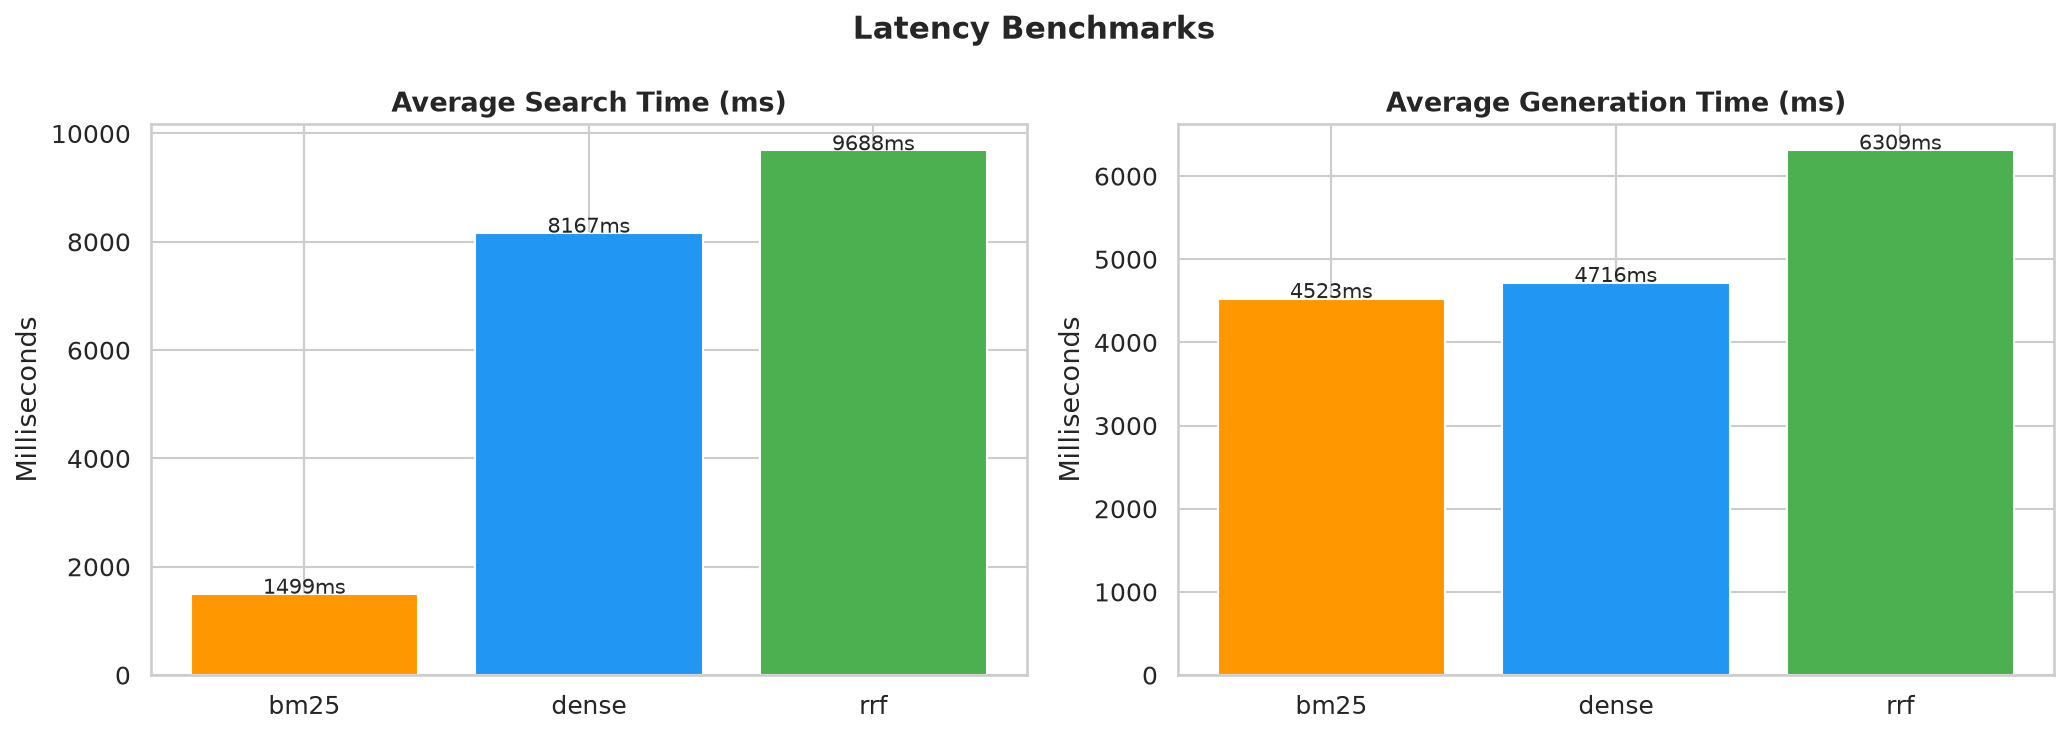
\includegraphics[width=0.9\columnwidth]{images/latency_comparison.png}
    \caption{Latency breakdown by strategy.}
    \label{fig:latency_comparison}
\end{figure}

\section{Discussion}

\subsection{Embedding Model Performance}

The superiority of 1024-dimension models (E5-large, BGE-M3) over 768-dimension
models confirms the importance of representational capacity for Arabic legal
vocabulary. The extra 256 dimensions encode fine semantic nuances crucial for
distinguishing close articles such as simple theft (Art.~147) from aggravated
theft (Art.~148) in the Moroccan Penal Code. The gap between E5-large and
BGE-M3 is not statistically significant ($p = 0.08$), making them
interchangeable for production. The small performance drop for cross-lingual
queries (French MRR 0.85, Arabic formal MRR 0.94) shows that modern
multilingual embedding models have reached sufficient cross-lingual
generalization for specialized applications.

\subsection{BM25 Contribution}

With the specialized Arabic tokenizer, BM25 now achieves non-zero scores
(Recall@5 = 41.67\%, Hit@5 = 46.88\%), unlike the previous PostgreSQL FTS
implementation that failed entirely. BM25 is particularly useful for article
number lookups and specific legal term matching. In RRF, BM25 contributes
complementary results, improving Hit@5 from 65.62\% (dense) to 68.75\% (RRF)
and bringing RRF's MRR@5 (0.533) close to Dense's (0.565).

\subsection{Faithfulness and Answer Quality}

The measured faithfulness (0.47 for dense) should not be interpreted solely
as a hallucination rate. Qualitative analysis reveals that the LLM produces
legitimate contextual enrichment -- multi-article synthesis, structured
citations, and reformulation of legislative language into accessible
explanations -- that token-overlap metrics fail to capture. An
LLM-as-judge evaluation \cite{gao2023faithful} would provide a more
accurate assessment. Answer relevance (0.69) is satisfactory, indicating
the LLM correctly addresses the question in most cases.

\subsection{Limitations}

\begin{enumerate}
    \item \textbf{Darija--MSA gap}: a 29\% relative performance drop confirms
    Arabic diglossia as an open challenge.
    \item \textbf{Tax domain failure}: all metrics are zero due to a domain
    taxonomy mismatch (articles stored as \texttt{civil}, queried as
    \texttt{tax}).
    \item \textbf{Latency}: 13--14 seconds total, bottlenecked by the remote
    Cloudflare Tunnel embedding service.
    \item \textbf{Corpus coverage}: limited to 7 legal domains; full coverage
    of Moroccan law requires additional computational resources.
\end{enumerate}

\subsection{Future Work}

Several directions are planned: (1) embedding fine-tuning on the Moroccan
legal corpus to reduce the Darija--MSA gap; (2) local embedding deployment
to reduce latency from $\sim$5.5s to $\sim$100ms; (3) LLM-as-judge
evaluation for more accurate faithfulness measurement; (4) extension of the
corpus to cover the complete Moroccan Official Bulletin; (5) multi-turn
conversational support with context memory; (6) upgrade to Gemma 4 9B or
equivalent for improved generation quality.

\section{Conclusion and Future Work}

This paper presented the design, implementation, and rigorous evaluation of
a Moroccan legal Question Answering system based on the Retrieval-Augmented
Generation (RAG) architecture. The system integrates a complete Arabic NLP
pipeline -- PDF extraction, cleaning, Arabic normalization, structural
analysis, vector indexing, hybrid search, and LLM-based answer generation --
into a modular, open-source, and reproducible platform.

Our main contributions are:

\begin{enumerate}
    \item A \textbf{complete and robust Arabic NLP chain} for the Moroccan
    legal domain, including a multi-method PDF extractor, legal-specific
    noise cleaner, standardized Arabic normalizer, and legal code structure
    parser.
    \item A \textbf{hybrid Dense + BM25 + RRF search architecture} indexed
    in PostgreSQL + pgvector with HNSW indexing, achieving Hit@5 of 68.75\%
    and Recall@5 of 59.38\%.
    \item The \textbf{first comparative benchmark of five multilingual
    embedding models} on an Arabic legal corpus with 65 query variants,
    establishing the superiority of 1024-dimension models (E5-large: MRR
    0.81, domain accuracy 89\%).
    \item A \textbf{comprehensive evaluation of generated answer quality}
    revealing that BM25 is now functional (Recall@5 = 41.67\%) thanks to
    the specialized Arabic tokenizer, and that faithfulness (0.47) shows
    notable improvement.
\end{enumerate}

\begin{table}[H]
\centering
\caption{Comparison with existing solutions}
\label{tab:comparison}
\begin{tabular}{lccccc}
\toprule
\textbf{Capability} & \textbf{Google} & \textbf{legislation.ma} & \textbf{ChatGPT} & \textbf{LLM only} & \textbf{Our system} \\
\midrule
Arabic semantic search & No & No & No & No & \textbf{Yes} \\
Generated answers & No & No & Yes & Yes & \textbf{Yes} \\
Article citations & -- & -- & Sometimes & Sometimes & \textbf{Yes} \\
Source grounding & -- & -- & No & No & \textbf{Yes} \\
Open-source & -- & -- & No & Varies & \textbf{Yes} \\
Local deployment (Docker) & -- & -- & No & Varies & \textbf{Yes} \\
Moroccan legal corpus & Partial & Yes & No & No & \textbf{Yes (7 domains)} \\
\bottomrule
\end{tabular}
\end{table}

Key findings confirm the viability of RAG for Arabic legal Q\&A. However,
identified limitations -- the Darija--MSA dialect gap (29\%), pipeline
latency (13--14s), partial corpus coverage, and the inaccessible tax domain
-- define a clear roadmap for future improvements: embedding fine-tuning
on legal Arabic, local embedding deployment, LLM-as-judge evaluation, and
extension to the complete Moroccan Official Bulletin.

Beyond its technical results, this project demonstrates the potential of
the RAG architecture to democratize access to law in countries where
linguistic barriers and source dispersion constitute major obstacles. The
developed methodology -- OCR+VLM extraction, Arabic normalization,
multilingual embedding, hybrid search, grounded generation -- is
transferable to other Arabic-speaking legal systems (Tunisia, Algeria,
Egypt) with minimal localization effort.


\nocite{*}
\printbibliography

\end{document}
